\chapter{Methodology}
\label{chap:methodology}



\section{System Design}
\label{sec:system-design}

Our neuro-symbolic planning system extends a re-implementation of the Generative Agents architecture \cite{parkGenerativeAgentsInteractive2023a} with modifications enabling controlled comparison between purely neural planning (baseline) and neuro-symbolic planning (our approach).

\subsection{System Architecture}
\label{subsec:system-architecture}

The implementation transforms the original monolithic Generative Agents codebase into a modular, service-oriented architecture:

\begin{enumerate}
    \item \textbf{Repository Layer}: Abstracts external dependencies (LLM APIs, file storage) behind interfaces. \texttt{LLMRepository} supports both OpenAI (production) and mock providers (testing). \texttt{EnvironmentRepository} abstracts world state persistence.

    \item \textbf{Service Layer}: Encapsulates cognitive capabilities in swappable interfaces:
          \begin{itemize}
              \item \texttt{PlanningService}: Daily planning and task decomposition
              \item \texttt{DialogueService}: Conversation generation
              \item \texttt{PerceptionService}: Environment observation and memory retrieval
              \item \texttt{ReflectionService}: Memory summarization
              \item \texttt{EnvironmentService}: Spatial navigation and object interaction
          \end{itemize}

    \item \textbf{Orchestration Layer}: The simulation loop consumes services through interfaces, configured via environment variables (\texttt{LLM\_PROVIDER}, \texttt{PLAN\_MODULE}) controlling which implementations run.
\end{enumerate}

\textbf{Key Design Principle}: The \texttt{PlanningService} abstraction enables side-by-side comparison of baseline (LLM-only hierarchical planning) and neuro-symbolic planning by ensuring both share identical environment state, memory retrieval, and LLM infrastructure. Only the planning logic differs, isolating the independent variable.

\begin{figure}[H]
    \centering
    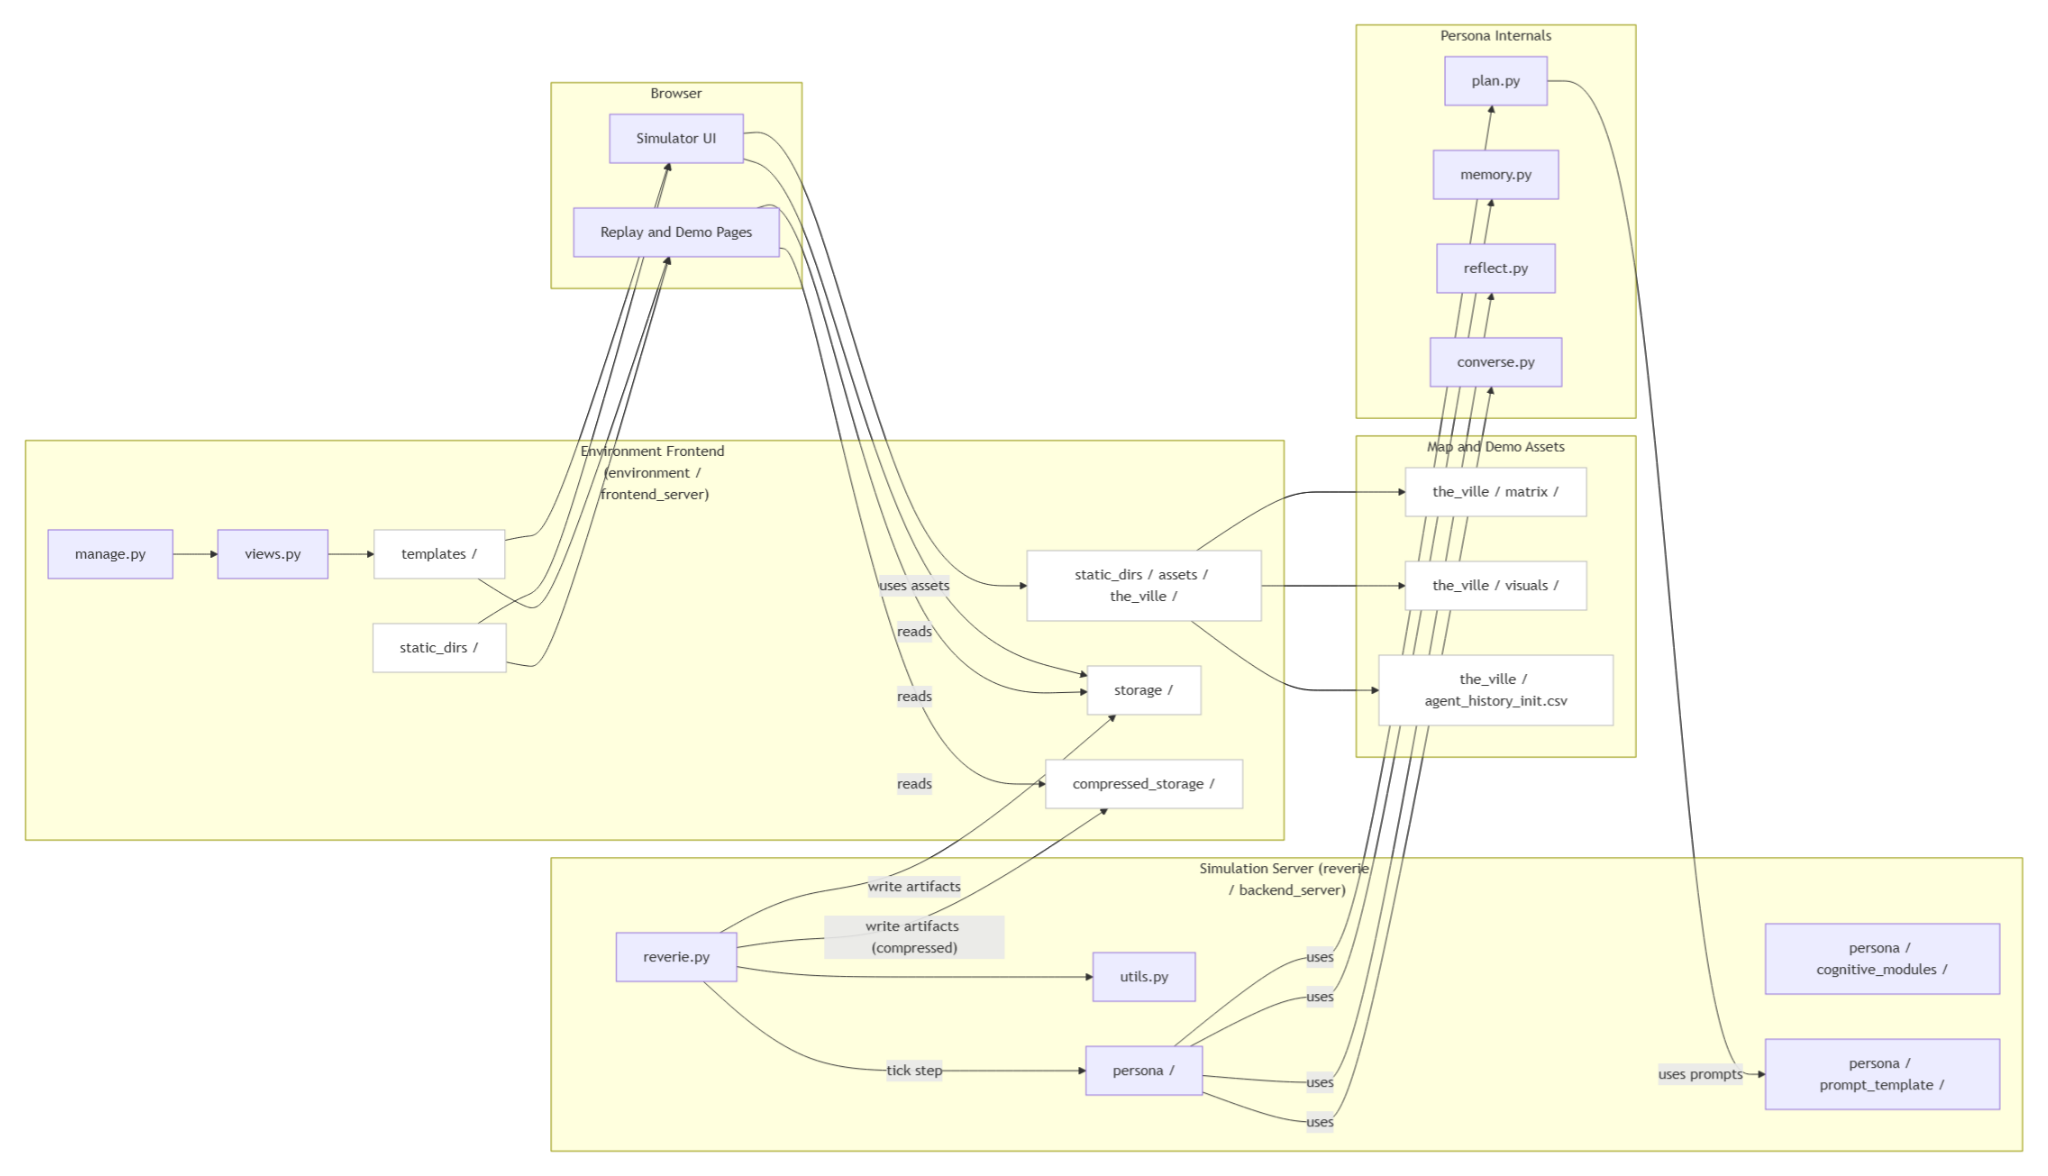
\includegraphics[width=\textwidth]{Pictures/Code Structure - before.png}
    \caption{Original monolithic architecture from the Generative Agents codebase \cite{parkGenerativeAgentsInteractive2023a}, showing tightly coupled components without clear separation of concerns.}
    \label{fig:code-structure-architecture-before}
\end{figure}

\begin{figure}[H]
    \centering
    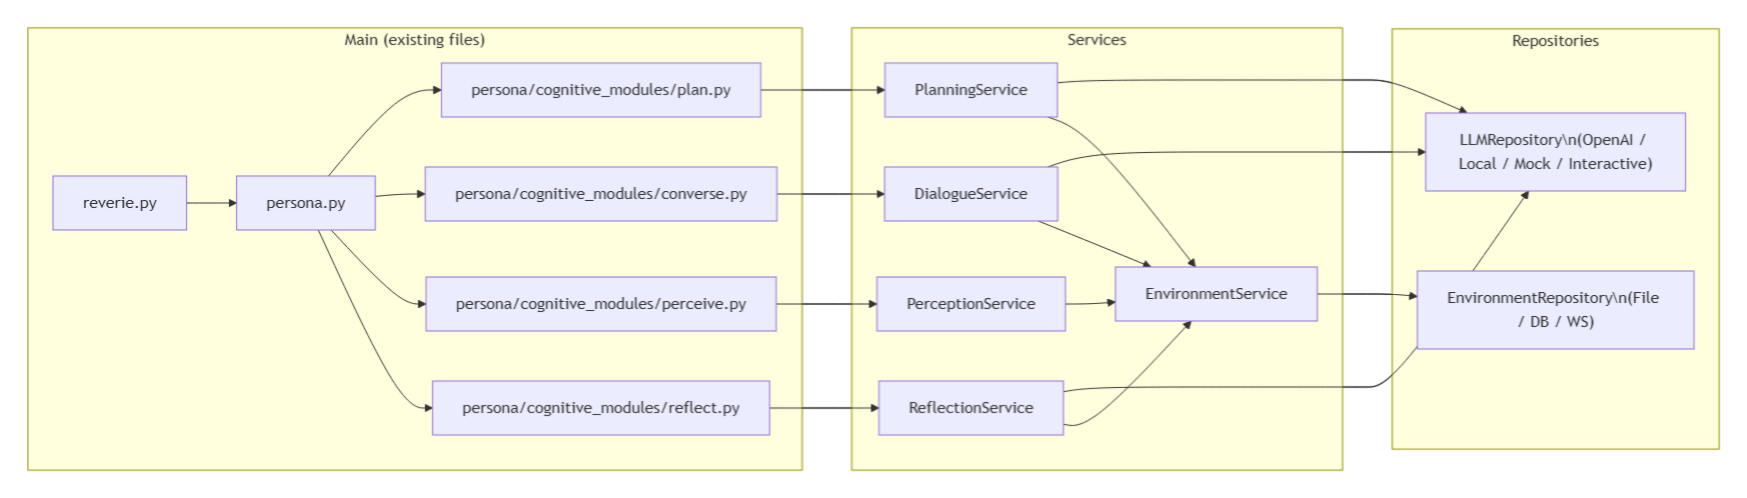
\includegraphics[width=\textwidth]{Pictures/Code Structure - after.png}
    \caption{Refactored service-oriented architecture with Repository, Service, and Orchestration layers. The \texttt{PlanningService} abstraction enables controlled comparison between baseline and neuro-symbolic planning implementations.}
    \label{fig:code-structure-architecture-after}
\end{figure}

\subsection{Prompt templetes}

\subsection{Long-term planning}

\subsubsection{Daily planning}
\subsubsection{Task decomposition}

\subsection{Movement}


\subsection{Neuro-Symbolic validation Pipeline}
\label{subsec:neuro-symbolic-pipeline}
We implemented following neuro-symbolic validation pipeline in hopes of enhancing coherence of actions generated as part of task decomposition [TODO add example] by checking validati of precondition by external symbolic vlaidation tool VAL. The feedback about validity of plan from VAL we need to generate 3 files Domain.pddl, Problem.pddl and plan.pddl bellow we explain how did we achive this.



\subsubsection{Domain generation}
Domain generation is the most difficult part of generation [Becouse it's the biggest mental load maybe add statistic for this. I mean it's just that domain need the most attention and problems here will propaget to following step of the pipeline] and we tested couple of aproches to do it correctly, bellow steps subjectivli [We tested a lot and look with genereted more sensible result and wich genereted less validation errors] generated the best Domain. We started with trying to generate the whole PDDL file in one go based on the decomposed action, but we got 2 problems 1. the actions conditions and effect tend to be chained without real logic to it. [add example, like teeth-brushed as precondition of shower]. So after many iteration we decided to split the domain generation into following steps.

    [ALso we use the structured JSON output to ensure proper naming and structure and we should write about it ]

\paragraph{Natural language precondition and effect generation}
We ask the model for nautal language condtions and effect of each action seperetly to prevent the chained condtion-effect problem that we observed when we genereting the whole domain in one go. [add example]

\paragraph{Predicates generation}
We gather all the natural language condition and effect of each action and world description and ask model to create a sensible predicate with focus on logic coherence. We do it in one go so we end up with unified set of predicate. As the domain is uniqe for specific agent and specific task decomposition we ask the model to generate zero arrity predicates as we saw that decrese amount of hallucination and malformated output from LLM's in the next stages of the pipeline [Add example]


\paragraph{PDDL Action schema generation }
Now for each action we generate action schema from the predicate catalog and natural language condtion and effects. We do it seperetly for each action to not encouraged the condtion and effect chaing. After that we programaticly create the domain file [Add example]

\paragraph{Validation with VAL and repair}
We check domain validation using VAL tool, The main porpus is to check out if model didn't Hallucinate new predicates or create othewise malfuntional PDDL schemas
Then I there is an error we pass the feedback to LLM that generated repaired domain [Add example]

\subsubsection{Problem generation}
After successfully generating the domian we ask LLM to generete the problem based on the predicates catalog current state of the world and the intenet of the task. form this we get initial state of the world and the goal. After generation the domain and problem file are feeded to VAL to check for syntax problems and potentialy hallucinations, and the problem is regenerated with VAL feedback in case of errors [Add example]

\subsubsection{Plan generation programmatic}
As we use zero arrity predicates then also the actions becomes zero arrity and becouse of that we can automatically generate the problem file from the original decomposed actions. [examples]

\subsubsection{VAL analysis}
We input the domain, problem and plan files to VAL and continue based on it feedback [add example] if the plan is valid we end the pipeline. If there are any error we move to a next step in the validaiton pipeline

\subsubsection{LLM feedback}
If there is error in VAL we input context of genereted PDDL artifact and feedback from VAL and ask LLM to generate actionable responses for each found errors. model can decide in between 1.Ok -can continue (when the error is becouse of not complete problem init state [Example there was no phone in the word state])
\texttt{pddl\_error} - There is error in pddl itself, [Add example]
\texttt{replan\_needed}
and based on all the error items, model decide one of 3 actions
ok - we end the pipeline and assume the the plan is valid
\texttt{pddl\_repair} - we repair each of the pddl artifact with feedback from VAL and then do VAL evaluation again
Replan needed - we continue with the pipeline

\subsubsection{Replan goal}
This stage creates an natural language replaning goal based on the feedback from validation and the current schedual, as well as task intent. We added this stage as we noticed that feeding PDDL feedback to replaner generetes poor results [examples]
\subsubsection{Replan}
In this stage we ask LLM to generate a new plan based on the replan goal, current schedual

we Repeat the above pipeline a set amount of times


\section{NL Condition Validation}
After validation pipeline We store the natural language preconditions for each action, so when the action begins we can check if the preconditions still hold and if the action is valid, so we can replan in case of broken condtions.
\subsection{Checking NL condition}
At begging of each action (when the agent actualy is about to execute the action), for each condition we retrive object state of the world around agent as well as other memories relevant to the conditions [EXAMPLE] and ask the model to based on that and commonsense categories the condition as satisfied or not. If all the condtions are satisfy agent will start the action
\subsection{Replan Goal}
If at least one of the condition is not satysfied we ask LLM to generate an replanning goal based on the schedual agent goal for a day and the violeted condtions. [example]
\subsection{Replan next 2h}
Then we ask LLM to replan the next 2h with the replan goal in mind[example]



\section{Quantitative Evaluation: Constraint Violation Analysis}
\label{sec:quantitative-evaluation}

[To be completed: automated evaluation comparing the hierarchical planning baseline against our validator-augmented system. The validator will automatically detect and flag constraint violations such as attempting to use items that are not available, scheduling overlapping activities, violating location constraints, or executing actions whose preconditions are not satisfied. Metrics will include violation counts at day-level and action-level, violation rates per 100 actions, and success rates after optional validator-guided repair rounds.]



\section{Experimental Setup}
\label{sec:experimental-setup}

[To be completed: overview of simulation environment, agent initialization, scenario design, and logging infrastructure.]


\section{User Study: Believability Evaluation}
\label{sec:user-study-believability}

This section describes the human-subjects study testing whether our approach improves perceived believability of agent behavior compared to the baseline Generative Agents architecture \cite{parkGenerativeAgentsInteractive2023a}. We focus on believability of \emph{actions} rather than only personalities or conversations.

\subsection{Objectives and Hypotheses}
\label{subsec:objectives-hypotheses}

Two primary hypotheses:

\begin{itemize}
    \item \textbf{H1 (overall believability)}: Participants judge agents powered by our method as more believable overall than the baseline in matched scenarios.
    \item \textbf{H2 (action believability)}: For the same scenario, participants flag fewer actions as ``unbelievable'' in our method than in the baseline.
\end{itemize}

Secondary outcomes: (i) perceived causal coherence when the high-level plan is visible, and (ii) free-text reasons participants provide when deeming actions unbelievable (used for qualitative error analysis) \cite{batesRoleEmotionBelievable1994,bogdanovychWhatMakesVirtual2016,tenceAutomatableEvaluationMethod2010,xiaoHowFarAre2024}.

\subsection{Conditions}
\label{subsec:conditions}

Two within-subject conditions on the same simulated world and character seeds:

\begin{enumerate}
    \item \textbf{Baseline (GA)}: Faithful re-implementation of Generative Agents \cite{parkGenerativeAgentsInteractive2023a}.
    \item \textbf{Ours (Neuro-symbolic)}: Proposed system with symbolic planning and consistency checks integrated into deliberation and action selection.
\end{enumerate}

Each participant evaluates both conditions on the same character and scenario to enable within-subject comparison. Order is counterbalanced to reduce presentation effects.

\subsection{Participants}
\label{subsec:participants}

Target 10 to 15 adult participants recruited from the university community and online platforms. Inclusion criteria: English proficiency. We run an initial pilot (3 to 4 participants) to validate timing and interface, then proceed to the main study. All participants provide informed consent and can withdraw anytime without penalty.

\subsection{Materials and Stimuli}
\label{subsec:materials-stimuli}

The stimulus for each condition is a replay of a single random character's day. To focus on action believability, we present:

\begin{itemize}
    \item time-lapse \emph{video replay} of the agent acting in the world (controllable playback speed, pause/seek);
    \item optional overlay with \emph{high-level plan} (intentions and sub-goals) and \emph{low-level action log}; and
    \item UI controls to mark an action as unbelievable (``thumbs down''), provide a short reason, and continue.
\end{itemize}

Replays cover the same scenario (e.g., two simulated in-game days) and use the same character profile and randomness seed across conditions, so any variation is attributable to agent architecture (baseline vs. ours) rather than scenario noise.

\subsection{Procedure}
\label{subsec:procedure}

Each session (approximately 30 minutes):

\begin{enumerate}
    \item \textbf{Introduction.} Scripted briefing introduces the task and believability as coherence, plausibility, and consistency within world rules \cite{bogdanovychWhatMakesVirtual2016}.
    \item \textbf{Practice.} Participants complete a 2 to 3 minute tutorial on the interface using a neutral example not used in the main study.
    \item \textbf{Condition A.} Watch the replay, freely scrub, and mark unbelievable actions. For each mark, add a short explanation (optional but encouraged).
    \item \textbf{Condition B.} Repeat with the other planner. Order varies across participants; assignment is double-blind.
    \item \textbf{Summary ratings.} For each condition: (i) overall believability rating (7-point Likert), (ii) perceived causal coherence rating (7-point Likert), and (iii) preference judgment (forced-choice which was more believable and why).
\end{enumerate}

We record duration until finished and whether the plan overlay was opened, to analyze how explanations affect believability judgments.

\subsection{Measures}
\label{subsec:measures}

We operationalize believability with participant-reported and behavior-linked measures. Higher values indicate higher believability unless noted.

\subsubsection{Primary Outcomes}
\label{subsubsec:primary-outcomes}

\begin{enumerate}
    \item \textbf{Overall believability (Likert).} Single item per condition on a 7-point scale: 1 ``not at all believable'', 4 ``moderately believable'', 7 ``extremely believable''. Prompt: ``How believable was the agent's behaviour overall in this replay?''

    \item \textbf{Action-level unbelievable rate (event-normalized).} Participants flag any action as unbelievable. Let $F$ be flagged action events and $A$ be \emph{atomic actions} viewed (from action log restricted to watched timestamps). The rate is
          \begin{equation}
              r_{\mathrm{unbel}} = \frac{F}{A} \times 100\,,
          \end{equation}
          expressed as flags per 100 atomic actions. Multiple flags within 2 seconds around the same atomic action merge into one.

    \item \textbf{Pairwise preference.} Forced-choice: ``Which replay was more believable overall?'' (Baseline vs. Ours).
\end{enumerate}

\subsubsection{Secondary Outcomes}
\label{subsubsec:secondary-outcomes}

\begin{itemize}
    \item \textbf{Causal coherence (Likert).} 7-point rating: 1 ``not coherent'', 7 ``highly coherent''.
    \item \textbf{Plan adherence (Likert).} 7-point rating of alignment between visible high-level plan and observed actions.
    \item \textbf{Unbelievable-action categories (coded).} Free-text reasons are open-coded into categories: goal inconsistency, environment rule violation, temporal implausibility, social norm violation, low-level control failure. Two independent coders label a stratified sample ($\geq 30\%$ of flags); disagreements are adjudicated and inter-rater agreement (Cohen's $\kappa$) is reported.
\end{itemize}

\textbf{Logged covariates (for analysis, not outcomes):} condition order, scenario ID, participant playback time, number of overlay openings, and self-reported prior experience with simulations/games. These are used as covariates in exploratory models and to check for order effects.

\subsection{Data Quality and Exclusion}
\label{subsec:data-quality}

Sessions are excluded if participants fail an attention check (simple comprehension question about the replay), leave more than half the session unanswered, or complete in less than one-third of median time. We pre-register exclusion rules prior to data collection.

\subsection{Ethics}
\label{subsec:ethics}

The study involves minimal risk. No personal data beyond demographics is collected; all logs are anonymized and stored on encrypted drives.
